
In the previous chapter, we studied the CPU resources and the ways to use them for optimal performance. In particular, we observed that CPUs have the ability to do quite a lot of computation in parallel (instruction-level parallelism). We demonstrated it on multiple benchmarks, which show that the CPU can do many operations per cycle without any performance penalty: adding and subtracting two numbers, for example, takes just as much time as only adding them.

You might have noticed, however, that these benchmarks and examples have one rather unusual property. Consider the following example:

\begin{lstlisting}[style=styleCXX]
for (size_t i = 0; i < N; ++i) {
	a1 += p1[i] + p2[i];
	a2 += p1[i] * p2[i];
	a3 += p1[i] << 2;
	a4 += p2[i] – p1[i];
	a5 += (p2[i] << 1)*p2[i];
	a6 += (p2[i] - 3)*p1[i];
}
\end{lstlisting}

We have already used this fragment of code to demonstrate that the CPU can do eight operations on the two values, p1[i] and p2[i], at almost no extra cost compared to just one operation. But we were always very careful to add more operations without adding more inputs; on several occasions, we mentioned, in passing, that the CPU's internal parallelism applies as long as the values are already in the registers. In the earlier example, while adding the second, third, and so on until the eighth operation, we were careful to stay with just two inputs. This results in some unusual and unrealistic code. In real life, how many things do you usually need to compute on a given set of inputs? Less than eight, most of the time.

This doesn't mean that the entire computational potential of the CPU is wasted unless you happen to run exotic code like the earlier example. The instruction-level parallelism is the computational foundation for pipelining, where we execute operations from different iterations of the loop simultaneously. Branchless computing is all about trading conditional instructions for unconditional computations and, therefore, relies almost entirely on the fact that we can usually get a few more computations for free.

The question remains, however: why did we limit our CPU benchmarks in this manner? After all, it would have been so much easier to come up with eight different things to do in the earlier example if we just added more inputs:

\begin{lstlisting}[style=styleCXX]
for (size_t i = 0; i < N; ++i) {
	a1 += p1[i] + p2[i];
	a2 += p3[i] * p4[i];
	a3 += p1[i] << 2;
	a4 += p2[i] - p3[i];
	a5 += (p4[i] << 1)*p2[i];
	a6 += (p3[i] - 3)*p1[i];
}
\end{lstlisting}

This is the same code as we saw earlier, only now it operates on four different input values per iteration instead of two. It does inherit all the awkwardness of the previous example, but only because we want to change as little as possible when measuring the impact of some change on performance. And the impact is significant:

\hspace*{\fill} \\ %插入空行
\begin{center}
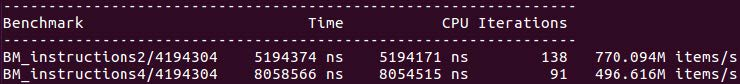
\includegraphics[width=0.9\textwidth]{content/1/chapter4/images/1.jpg}\\
Figure 4.1
\end{center}

The same computations done on four input values take about 36\% longer. The computations are delayed, somehow, when we need to access more data in memory.

It should be noted that there is another reason why adding more independent variables, inputs, or outputs, could impact the performance: the CPU could be running out of registers in which to store these variables for computations. While this is a significant concern in many real programs, it is not the case here. The code isn't complex enough to use up all the registers of a modern CPU (the easiest way to confirm this is by examining the machine code, unfortunately).

Clearly, accessing more data seems to reduce the speed of the code. But why? At a very high level, the reason is that the memory simply cannot keep up with the CPU. There are several ways to estimate the size of this memory gap. The simplest way is evident in the specs of a modern CPU. CPUs today operate at clock frequencies between 3 GHz and 4 GHz, which means that one cycle is about 0.3 nanoseconds. As we have seen, under the right circumstances, the CPU can do several operations per second, so executing ten operations per nanosecond is not out of the question (although hard to achieve in practice and is a sure sign of a very efficient program). On the other hand, the memories are much slower: the DDR4 memory clock, for example, operates at 400 MHz. You can also find the values as high as 3200 MHz; however, this is not the memory clock but the data rate, and to convert it to something resembling memory speed, you also have to take into account the Column Access Strobe Latency, usually known as CAS Latency or CL. Roughly, this is the number of cycles it takes for the RAM to receive a request for data, process it, and return the value. There is no single definition of memory speed that makes sense under all circumstances (later in this chapter, we will see some of the reasons why), but, to the first approximation, the memory speed of a DDR4 module with the data rate of 3.2 GHz and CAS Latency 15 is about 107 MHz or 9.4 nanoseconds per access.

Whichever way you look at it, the CPU can do a lot more operations per second than the memory can supply the input values for these operations or store the results. All programs need to use memory in some way, and the details of how the memory is accessed are going to have a significant impact on performance, sometimes to the point of limiting it. The details, however, are extremely important: the effects of the memory gap on performance can vary from insignificant to memory becoming the bottleneck of the program. We have to understand how the memory impacts the program performance under different conditions and why, so we can use this knowledge to design and implement our code for the best performance.








